\section{Git Basics}

\begin{frame}{What Do We Know So Far?}
  \begin{itemize}
    \item Initialize a repository
    \item Clone a repository
    \item Save changes (commit)
    \item Upload changes to the remote repository (push)
    \item Download the latest changes from the repository (pull)
    \item What else to acquire?
    \begin{itemize}
        \item Create a branch
        \item Switch to branch
        \item Merge branches and solve conflicts
    \end{itemize}
  \end{itemize}
\end{frame}

\section{Branching in Git}

\begin{frame}{What is a Branch?}
  \begin{itemize}
    \item A branch is a line of development.
    \item A project can have multiple lines of development in parallel.
    \item Common branches:
      \begin{itemize}
        \item \textbf{Main}: Contains the last stable version.
        \item \textbf{Devel}: Contains the next candidate for a stable version.
        \item \textbf{Feature branches}: Each task/feature is developed in a separate branch.
      \end{itemize}
  \end{itemize}
  
  \centering
  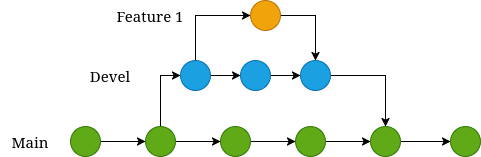
\includegraphics[width=0.5\linewidth]{trainingmaterials/git-II/rpi_upm.branches.png }
\end{frame}

\begin{frame}{Using Branches}
  \begin{itemize}
    \item To create a new branch:
      \begin{itemize}
        \item \texttt{git checkout -b <branch\_name>}
      \end{itemize}
    \item To switch to an existing branch:
      \begin{itemize}
        \item \texttt{git checkout <branch\_name>}
      \end{itemize}
    \item Remember to specify the branch name when pushing:
      \begin{itemize}
        \item \texttt{git push origin <branch\_name>}
      \end{itemize}
    \item Useful command to check the current branch and working area status:
      \begin{itemize}
        \item \texttt{git status}
      \end{itemize}
    \item Useful command to check the history of a branch:
      \begin{itemize}
        \item \texttt{git log}
      \end{itemize}
  \end{itemize}
\end{frame}

\begin{frame}{Using Branches Example}
  \centering
  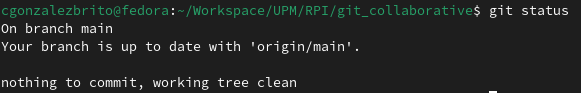
\includegraphics[width=0.75\linewidth]{trainingmaterials/git-II/git_status_main.png}
  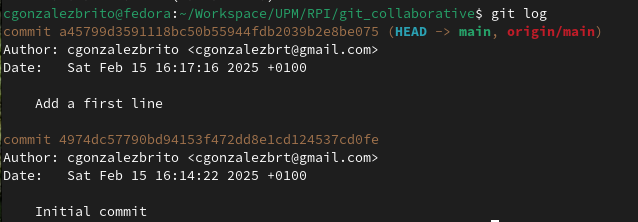
\includegraphics[width=0.75\linewidth]{trainingmaterials/git-II/git_log_main.png}
  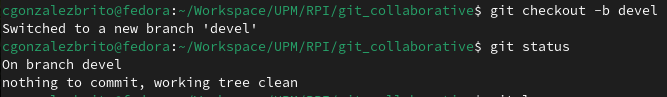
\includegraphics[width=0.75\linewidth]{trainingmaterials/git-II/git_new_branch_devel.png}
\end{frame}


\begin{frame}{Using Branches Example II}
  \centering
  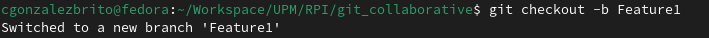
\includegraphics[width=0.75\linewidth]{trainingmaterials/git-II/git_new_branch_feature1.png}
  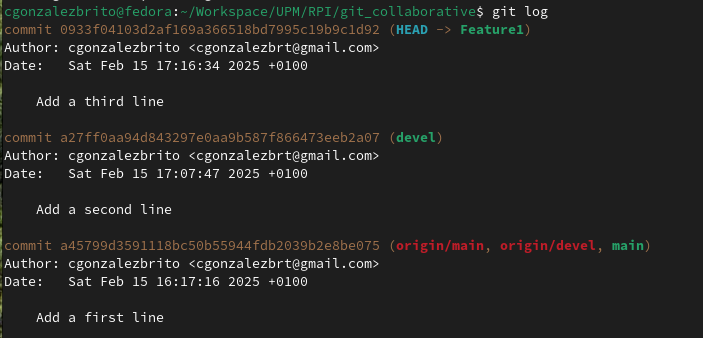
\includegraphics[width=0.75\linewidth]{trainingmaterials/git-II/git_log_feature.png}
\end{frame}

\section{Merging and Conflict Resolution}

\begin{frame}{Merging Branches}
  \begin{itemize}
    \item When work is finished, merge the changes from your branch into \texttt{devel}.
    \item Procedure: 
        \begin{enumerate}
            \item Switch to \texttt{devel} branch: \texttt{git checkout devel}
            \item Update \texttt{devel} branch: \texttt{git pull origin devel}
            \item Merge your branch into \texttt{devel}: \texttt{git merge <branch\_name>}
      \end{enumerate}
  \end{itemize}
  
  \centering
  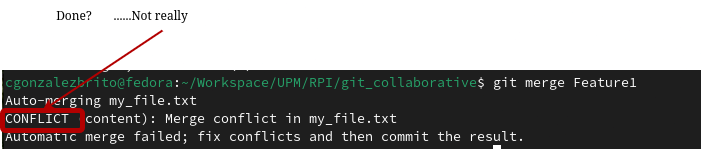
\includegraphics[width=0.75\linewidth]{trainingmaterials/git-II/git_merge_conflict.png}
\end{frame}

\begin{frame}{Handling Conflicts}
  \begin{itemize}
    \item Git automatically merges changes, but conflicts can occur when:
      \begin{itemize}
        \item Different developers make changes in the same place of a document.
      \end{itemize}
  \end{itemize}
  \centering
  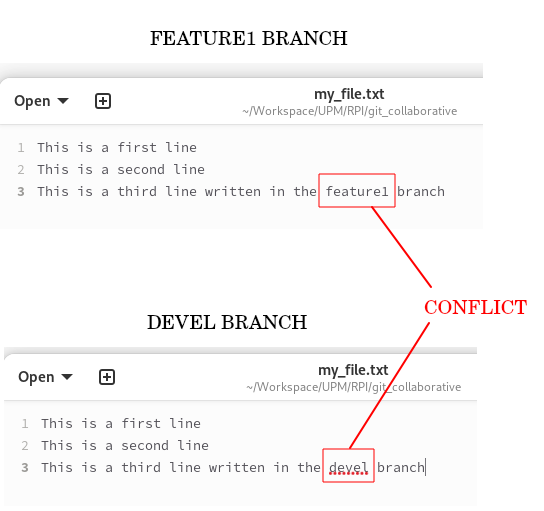
\includegraphics[width=0.5\linewidth]{trainingmaterials/git-II/conflict.png}
\end{frame}

\begin{frame}{Handling Conflicts II}
  \begin{itemize}
    \item To resolve conflicts:
      \begin{enumerate}
        \item Install \texttt{meld}.
        \item Run \texttt{git mergetool}.
        \item Inspect the files and resolve conflicts by:
          \begin{itemize}
            \item Using all local changes.
            \item Using all remote changes.
            \item Mixing changes as needed.
          \end{itemize}
        \item Save, commit, and push the resolved changes.
      \end{enumerate}
  \end{itemize}
  \centering
  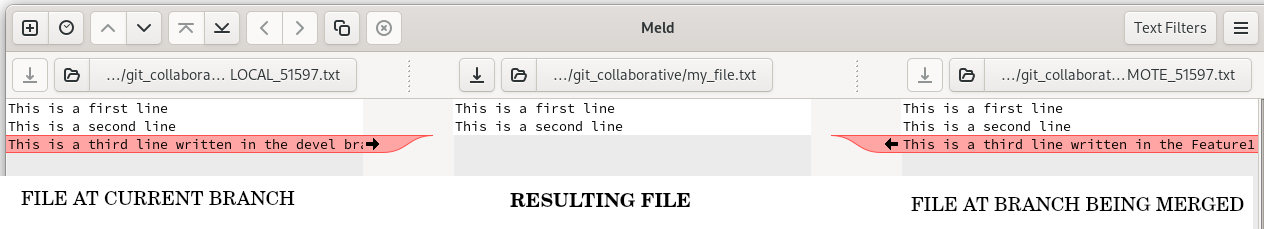
\includegraphics[width=1\linewidth]{trainingmaterials/git-II/meld.png}
\end{frame}

\begin{frame}{Best Practices}
  \begin{itemize}
    \item Use a Git cheatsheet for quick reference: \href{https://ndpsoftware.com/git-cheatsheet.html}{"Git Cheatsheet"}
    \item Before pulling or pushing, synchronize your local repository index with the remote using:
      \begin{itemize}
        \item \texttt{git fetch}
      \end{itemize}
    \item Merge \texttt{devel} into your branch before merging your branch into \texttt{devel} to:
      \begin{itemize}
        \item Fix conflicts.
        \item Test that everything works as expected.
        \item Ensure a conflict-free merge into \texttt{devel}.
      \end{itemize}
    \item Write meaningful commit messages:
      \begin{itemize}
        \item First line: Brief summary.
        \item Following lines: Detailed explanation of changes (if required).
      \end{itemize}
    \item Push only tested code to \texttt{devel} and stable versions to \texttt{main}.
  \end{itemize}
\end{frame}

\section{Quick Guide}

\begin{frame}{Working with Feature Branches}
  \begin{itemize}
    \item Clone repository and create a feature branch:
      \begin{itemize}
        \item \texttt{git clone <repository\_url>}
        \item \texttt{git checkout -b <feature\_branch>}
      \end{itemize}
    \item Develop and test your feature.
    \item Commit changes with a message:
      \begin{itemize}
        \item \texttt{git commit -m "Message"}
      \end{itemize}
    \item Fetch and pull the latest changes:
      \begin{itemize}
        \item \texttt{git fetch}
        \item \texttt{git pull origin <feature\_branch>}
      \end{itemize}
    \item Resolve conflicts, if any.
    \item Push your changes:
      \begin{itemize}
        \item \texttt{git push origin <feature\_branch>}
      \end{itemize}
  \end{itemize}
\end{frame}

\begin{frame}{Merging Feature Branch into \texttt{devel}}
  \begin{itemize}
    \item Switch to \texttt{devel} branch:
      \begin{itemize}
        \item \texttt{git checkout devel}
      \end{itemize}
    \item Fetch and pull the latest changes:
      \begin{itemize}
        \item \texttt{git fetch}
        \item \texttt{git pull origin devel}
      \end{itemize}
    \item Merge \texttt{devel} into your feature branch:
      \begin{itemize}
        \item \texttt{git checkout <feature\_branch>}
        \item \texttt{git merge devel}
      \end{itemize}
    \item Resolve conflicts
   \end{itemize}
\end{frame}
 

